\documentclass{ximera}

%\usepackage{todonotes}
%\usepackage{mathtools} %% Required for wide table Curl and Greens
%\usepackage{cuted} %% Required for wide table Curl and Greens
\newcommand{\todo}{}

\usepackage{esint} % for \oiint
\ifxake%%https://math.meta.stackexchange.com/questions/9973/how-do-you-render-a-closed-surface-double-integral
\renewcommand{\oiint}{{\large\bigcirc}\kern-1.56em\iint}
\fi


\graphicspath{
  {./}
  {ximeraTutorial/}
  {basicPhilosophy/}
  {functionsOfSeveralVariables/}
  {normalVectors/}
  {lagrangeMultipliers/}
  {vectorFields/}
  {greensTheorem/}
  {shapeOfThingsToCome/}
  {dotProducts/}
  {partialDerivativesAndTheGradientVector/}
  {../productAndQuotientRules/exercises/}
  {../normalVectors/exercisesParametricPlots/}
  {../continuityOfFunctionsOfSeveralVariables/exercises/}
  {../partialDerivativesAndTheGradientVector/exercises/}
  {../directionalDerivativeAndChainRule/exercises/}
  {../commonCoordinates/exercisesCylindricalCoordinates/}
  {../commonCoordinates/exercisesSphericalCoordinates/}
  {../greensTheorem/exercisesCurlAndLineIntegrals/}
  {../greensTheorem/exercisesDivergenceAndLineIntegrals/}
  {../shapeOfThingsToCome/exercisesDivergenceTheorem/}
  {../greensTheorem/}
  {../shapeOfThingsToCome/}
  {../separableDifferentialEquations/exercises/}
  {vectorFields/}
}

\newcommand{\mooculus}{\textsf{\textbf{MOOC}\textnormal{\textsf{ULUS}}}}

\usepackage{tkz-euclide}\usepackage{tikz}
\usepackage{tikz-cd}
\usetikzlibrary{arrows}
\tikzset{>=stealth,commutative diagrams/.cd,
  arrow style=tikz,diagrams={>=stealth}} %% cool arrow head
\tikzset{shorten <>/.style={ shorten >=#1, shorten <=#1 } } %% allows shorter vectors

\usetikzlibrary{backgrounds} %% for boxes around graphs
\usetikzlibrary{shapes,positioning}  %% Clouds and stars
\usetikzlibrary{matrix} %% for matrix
\usepgfplotslibrary{polar} %% for polar plots
\usepgfplotslibrary{fillbetween} %% to shade area between curves in TikZ
\usetkzobj{all}
\usepackage[makeroom]{cancel} %% for strike outs
%\usepackage{mathtools} %% for pretty underbrace % Breaks Ximera
%\usepackage{multicol}
\usepackage{pgffor} %% required for integral for loops



%% http://tex.stackexchange.com/questions/66490/drawing-a-tikz-arc-specifying-the-center
%% Draws beach ball
\tikzset{pics/carc/.style args={#1:#2:#3}{code={\draw[pic actions] (#1:#3) arc(#1:#2:#3);}}}



\usepackage{array}
\setlength{\extrarowheight}{+.1cm}
\newdimen\digitwidth
\settowidth\digitwidth{9}
\def\divrule#1#2{
\noalign{\moveright#1\digitwidth
\vbox{\hrule width#2\digitwidth}}}





\newcommand{\RR}{\mathbb R}
\newcommand{\R}{\mathbb R}
\newcommand{\N}{\mathbb N}
\newcommand{\Z}{\mathbb Z}

\newcommand{\sagemath}{\textsf{SageMath}}


%\renewcommand{\d}{\,d\!}
\renewcommand{\d}{\mathop{}\!d}
\newcommand{\dd}[2][]{\frac{\d #1}{\d #2}}
\newcommand{\pp}[2][]{\frac{\partial #1}{\partial #2}}
\renewcommand{\l}{\ell}
\newcommand{\ddx}{\frac{d}{\d x}}

\newcommand{\zeroOverZero}{\ensuremath{\boldsymbol{\tfrac{0}{0}}}}
\newcommand{\inftyOverInfty}{\ensuremath{\boldsymbol{\tfrac{\infty}{\infty}}}}
\newcommand{\zeroOverInfty}{\ensuremath{\boldsymbol{\tfrac{0}{\infty}}}}
\newcommand{\zeroTimesInfty}{\ensuremath{\small\boldsymbol{0\cdot \infty}}}
\newcommand{\inftyMinusInfty}{\ensuremath{\small\boldsymbol{\infty - \infty}}}
\newcommand{\oneToInfty}{\ensuremath{\boldsymbol{1^\infty}}}
\newcommand{\zeroToZero}{\ensuremath{\boldsymbol{0^0}}}
\newcommand{\inftyToZero}{\ensuremath{\boldsymbol{\infty^0}}}



\newcommand{\numOverZero}{\ensuremath{\boldsymbol{\tfrac{\#}{0}}}}
\newcommand{\dfn}{\textbf}
%\newcommand{\unit}{\,\mathrm}
\newcommand{\unit}{\mathop{}\!\mathrm}
\newcommand{\eval}[1]{\bigg[ #1 \bigg]}
\newcommand{\seq}[1]{\left( #1 \right)}
\renewcommand{\epsilon}{\varepsilon}
\renewcommand{\phi}{\varphi}


\renewcommand{\iff}{\Leftrightarrow}

\DeclareMathOperator{\arccot}{arccot}
\DeclareMathOperator{\arcsec}{arcsec}
\DeclareMathOperator{\arccsc}{arccsc}
\DeclareMathOperator{\si}{Si}
\DeclareMathOperator{\scal}{scal}
\DeclareMathOperator{\sign}{sign}


%% \newcommand{\tightoverset}[2]{% for arrow vec
%%   \mathop{#2}\limits^{\vbox to -.5ex{\kern-0.75ex\hbox{$#1$}\vss}}}
\newcommand{\arrowvec}[1]{{\overset{\rightharpoonup}{#1}}}
%\renewcommand{\vec}[1]{\arrowvec{\mathbf{#1}}}
\renewcommand{\vec}[1]{{\overset{\boldsymbol{\rightharpoonup}}{\mathbf{#1}}}\hspace{0in}}

\newcommand{\point}[1]{\left(#1\right)} %this allows \vector{ to be changed to \vector{ with a quick find and replace
\newcommand{\pt}[1]{\mathbf{#1}} %this allows \vec{ to be changed to \vec{ with a quick find and replace
\newcommand{\Lim}[2]{\lim_{\point{#1} \to \point{#2}}} %Bart, I changed this to point since I want to use it.  It runs through both of the exercise and exerciseE files in limits section, which is why it was in each document to start with.

\DeclareMathOperator{\proj}{\mathbf{proj}}
\newcommand{\veci}{{\boldsymbol{\hat{\imath}}}}
\newcommand{\vecj}{{\boldsymbol{\hat{\jmath}}}}
\newcommand{\veck}{{\boldsymbol{\hat{k}}}}
\newcommand{\vecl}{\vec{\boldsymbol{\l}}}
\newcommand{\uvec}[1]{\mathbf{\hat{#1}}}
\newcommand{\utan}{\mathbf{\hat{t}}}
\newcommand{\unormal}{\mathbf{\hat{n}}}
\newcommand{\ubinormal}{\mathbf{\hat{b}}}

\newcommand{\dotp}{\bullet}
\newcommand{\cross}{\boldsymbol\times}
\newcommand{\grad}{\boldsymbol\nabla}
\newcommand{\divergence}{\grad\dotp}
\newcommand{\curl}{\grad\cross}
%\DeclareMathOperator{\divergence}{divergence}
%\DeclareMathOperator{\curl}[1]{\grad\cross #1}
\newcommand{\lto}{\mathop{\longrightarrow\,}\limits}

\renewcommand{\bar}{\overline}

\colorlet{textColor}{black}
\colorlet{background}{white}
\colorlet{penColor}{blue!50!black} % Color of a curve in a plot
\colorlet{penColor2}{red!50!black}% Color of a curve in a plot
\colorlet{penColor3}{red!50!blue} % Color of a curve in a plot
\colorlet{penColor4}{green!50!black} % Color of a curve in a plot
\colorlet{penColor5}{orange!80!black} % Color of a curve in a plot
\colorlet{penColor6}{yellow!70!black} % Color of a curve in a plot
\colorlet{fill1}{penColor!20} % Color of fill in a plot
\colorlet{fill2}{penColor2!20} % Color of fill in a plot
\colorlet{fillp}{fill1} % Color of positive area
\colorlet{filln}{penColor2!20} % Color of negative area
\colorlet{fill3}{penColor3!20} % Fill
\colorlet{fill4}{penColor4!20} % Fill
\colorlet{fill5}{penColor5!20} % Fill
\colorlet{gridColor}{gray!50} % Color of grid in a plot

\newcommand{\surfaceColor}{violet}
\newcommand{\surfaceColorTwo}{redyellow}
\newcommand{\sliceColor}{greenyellow}




\pgfmathdeclarefunction{gauss}{2}{% gives gaussian
  \pgfmathparse{1/(#2*sqrt(2*pi))*exp(-((x-#1)^2)/(2*#2^2))}%
}


%%%%%%%%%%%%%
%% Vectors
%%%%%%%%%%%%%

%% Simple horiz vectors
\renewcommand{\vector}[1]{\left\langle #1\right\rangle}


%% %% Complex Horiz Vectors with angle brackets
%% \makeatletter
%% \renewcommand{\vector}[2][ , ]{\left\langle%
%%   \def\nextitem{\def\nextitem{#1}}%
%%   \@for \el:=#2\do{\nextitem\el}\right\rangle%
%% }
%% \makeatother

%% %% Vertical Vectors
%% \def\vector#1{\begin{bmatrix}\vecListA#1,,\end{bmatrix}}
%% \def\vecListA#1,{\if,#1,\else #1\cr \expandafter \vecListA \fi}

%%%%%%%%%%%%%
%% End of vectors
%%%%%%%%%%%%%

%\newcommand{\fullwidth}{}
%\newcommand{\normalwidth}{}



%% makes a snazzy t-chart for evaluating functions
%\newenvironment{tchart}{\rowcolors{2}{}{background!90!textColor}\array}{\endarray}

%%This is to help with formatting on future title pages.
\newenvironment{sectionOutcomes}{}{}



%% Flowchart stuff
%\tikzstyle{startstop} = [rectangle, rounded corners, minimum width=3cm, minimum height=1cm,text centered, draw=black]
%\tikzstyle{question} = [rectangle, minimum width=3cm, minimum height=1cm, text centered, draw=black]
%\tikzstyle{decision} = [trapezium, trapezium left angle=70, trapezium right angle=110, minimum width=3cm, minimum height=1cm, text centered, draw=black]
%\tikzstyle{question} = [rectangle, rounded corners, minimum width=3cm, minimum height=1cm,text centered, draw=black]
%\tikzstyle{process} = [rectangle, minimum width=3cm, minimum height=1cm, text centered, draw=black]
%\tikzstyle{decision} = [trapezium, trapezium left angle=70, trapezium right angle=110, minimum width=3cm, minimum height=1cm, text centered, draw=black]


\outcome{Understand how divergence measures local expansion.}
\outcome{Understand that divergence need not measure gobal expansion.}
\outcome{Compute the flow of a vector field across a curve.}
\outcome{State the flux form of Green's Theorem.}

\title[Dig-In:]{Divergence and line integrals}

\begin{document}
\begin{abstract}
  Divergence measures the rate field vectors are expanding at a point.
\end{abstract}
\maketitle

While the gradient and curl are the fundamental ``derivatives'' in two
dimensions, there is another useful measurement we can make. It is
called \textit{divergence}. It measures the rate field vectors are
``expanding'' at a given point.

\section{The divergence of a vector field}

Let's state the definition:

\begin{definition}
  Given a vector field $\vec{F}:\R^n\to \R^n$, where
  \[
  \vec{F}(x_1,\dots,x_n) = \begin{bmatrix}
    M_1(x_1,\dots,x_n)\\
    M_2(x_1,\dots,x_n)\\
    \vdots \\
    M_n(x_1,\dots,x_n)
  \end{bmatrix}
  \]
  the \dfn{divergence} is given by
  \[
  \divergence \vec F =\pp[M_1]{x_1} + \pp[M_2]{x_2} + \dots + \pp[M_n]{x_n}. 
  \]
\end{definition}

\begin{question}
  The divergence of a vector field is a \dots
  \begin{multipleChoice}
    \choice{vector.}
    \choice[correct]{scalar.}
    \choice{neither a vector nor a scalar.}
  \end{multipleChoice}
  \begin{feedback}
    The divergence is a number that tells you how much the field is
    expanding at a point. However, no directional information is
    given.
  \end{feedback}
\end{question}

\begin{question}
  Consider the vector field $\vec{F}(x,y) =
  \vector{x^2y^3,ye^x}$. Compute:
  \[
  \divergence\vec{F}
  \begin{prompt}
    = \answer{2xy^3 + e^x}
  \end{prompt}
  \]
  \begin{question}
    Consider the vector field $\vec{F}(x,y,z) =
    \vector{\sin(xy),\sin(x+y+z),\sin(yz}$. Compute:
    \[
    \divergence\vec{F}
    \begin{prompt}
    = \answer{y\cos(xy) + \cos(x+y+z) + y\cos(yz)}
    \end{prompt}
    \]
  \end{question}
\end{question}

\subsection{What does divergence measure?}

As we've already said, divergence measures the rate field vectors are
expanding at a point. The most obvious example of a vector field with
nonzero divergence is $\vec{F}(x,y)= \vector{x,y}$
\begin{image}
  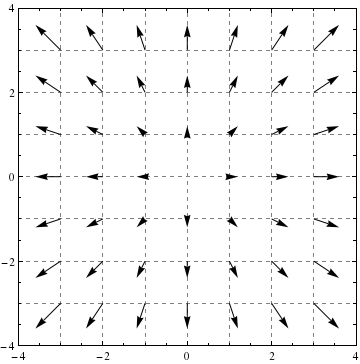
\includegraphics{divField.png}
\end{image}
On the other hand, recall that a \dfn{radial} vector field is a field
of the form $\vec{F}:\R^n\to\R^n$ where
\[
\vec{F}(\vec{x}) = \frac{\pm\vec{x}}{|\vec{x}|^p}
\]
where $p$ is a real number. The divergence of these vector fields can
be surprising.

\begin{example}
  Compute the divergence of $\vec{F}(x,y) =\frac{\vector{x,y}}{|\vector{x,y}|^p}$.
    \begin{explanation}
      First note
      \begin{align*}
        \pp{x} \frac{x}{(\sqrt{x^2+y^2})^p} &= \pp{x} \frac{x}{(x^2+y^2)^{p/2}} \\
        &= \answer[given]{\frac{(x^2+y^2)^{p/2}-px^2 (x^2+y^2)^{p/2-1}}{(x^2+y^2)^p}}
      \end{align*}
      and next note
      \begin{align*}
        \pp{y} \frac{y}{(\sqrt{x^2+y^2})^p} &= \pp{y} \frac{y}{(x^2+y^2)^{p/2}} \\
        &= \answer[given]{\frac{(x^2+y^2)^{p/2}-py^2 (x^2+y^2)^{p/2-1}}{(x^2+y^2)^p}}
      \end{align*}
      so
      \begin{align*}
        \divergence\vec{F}(x,y) = \frac{2-p}{|\vector{x,y}|^p}
      \end{align*}
    \end{explanation}
\end{example}

\begin{question}
  Compute the divergence of $\vec{F} =\frac{\vector{x,y,z}}{|\vector{x,y,z}|^p}$.
  \begin{prompt}
    \[
    \divergence\vec{F}(x,y,z) = \frac{\answer[given]{3-p}}{|\vector{x,y,z}|^p}
    \]
  \end{prompt}
\end{question}

Now we will see a radial vector field with zero divergence.

\begin{example}
  Consider the vector field $\vec{F}(x,y) =
  \frac{\vector{x,y}}{|\vector{x,y}|^2}$:
  \begin{image}
    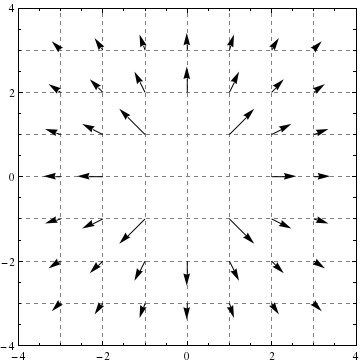
\includegraphics{divFieldZero.png}
  \end{image}
  Compute $\divergence\vec{F}$.
  \begin{explanation}
    Since this is a radial field, we know its divergence is
    \[
    \frac{2-\answer[given]{2}}{|\vector{x,y}|^p} = \answer[given]{0}
    \]
    when $\vector{x,y}\ne\vec{0}$.
  \end{explanation}
\end{example}

Now let's see a radial vector field with negative divergence.

\begin{example}
  Consider the vector field $\vec{F}(x,y) =
  \frac{\vector{x,y}}{|\vector{x,y}|^3}$:
  \begin{image}
    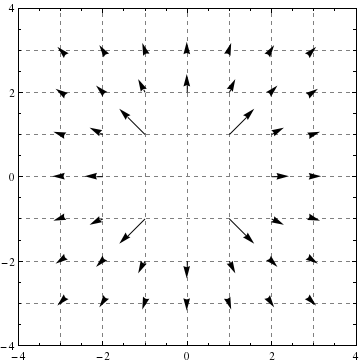
\includegraphics{divFieldNeg.png}
  \end{image}
  Compute $\divergence\vec{F}$.
  \begin{explanation}
    Since this is a radial field, we know its divergence is
    \[
    \frac{2-\answer[given]{3}}{|\vector{x,y}|^p} < 0
    \]
    when $\vector{x,y}\ne\vec{0}$.
  \end{explanation}
\end{example}

\section{Measuring flow across a curve}

Let $\vec{F}:\R^2\to\R^2$ be a vector field,
$\vec{p}:\R\to\R^2$ be a smooth vector valued function tracing a curve
$C$ exactly once as $t$ runs from $a$ to $b$,
\begin{align*}
  \vec{F}(x,y) &= \vector{M(x,y), N(x,y)}\\
  \vec{p}(t) &= \vector{x(t),y(t)}.
\end{align*}
Recall that the line integral
\[
\int_C \vec{F}\dotp\d\vec{p}
\]
measures the accumulated flow of a vector field along a curve. We see
this because $\vec{F}\dotp\vec{p}'$ measures how ``aligned'' field
vectors are with the direction of the path $\vec{p}$. On the other
hand, if we set
\[
\vec{n}(t) = \vector{y(t),-x(t)}
\]
then for any given value of $t$, $\vec{n}'(t)$ is a vector that is
orthogonal to $\vec{p}'(t)$. Moreover, given a closed curve, where
$\vec{p}(t)$ is parameterized with the interior on the left,
$\vec{n}'(t)$ points outward. Below we see a curve $\vec{p}(t)$ along
with some tangent vectors $\vec{p}'(t)$ and some outward normal
vectors $\vec{n}'(t)$:
\begin{image}
    \begin{tikzpicture}
      \begin{axis}%
        [
	  ymin=-4,ymax=7,
	  xmin=-7,xmax=7,
          axis lines =middle, xlabel=$x$, ylabel=$y$,
          every axis y label/.style={at=(current axis.above origin),anchor=south},
          every axis x label/.style={at=(current axis.right of origin),anchor=west},
          grid=both,
          grid style={dashed, gridColor},
	]
        \addplot[penColor2,ultra thick,smooth] coordinates{
          (0,-1) (2,-2) (4,0) (4,2) (3,3) (1,4)
          (-1,5) (-3,4) (-4,2.5) (-4,1) (-2,0) (0,-1)
        };
        \fill[black,draw=black] (axis cs:1,4) circle (2.5pt);
        \fill[black,draw=black] (axis cs:-2,0) circle (2.5pt);
        \fill[black,draw=black] (axis cs:4,2) circle (2.5pt);
        \fill[black,draw=black] (axis cs:-4,2.5) circle (2.5pt);

        \addplot[penColor,thick,->] coordinates{
          (1,4) (-2,5.7) 
        };
        \addplot[penColor4,thick,->] coordinates{
          (1,4) (2.7,7) 
        };

      
        \addplot[penColor,thick,->] coordinates{
          (4,2) (3,4) 
        };
        \addplot[penColor4,thick,->] coordinates{
          (4,2) (6,3) 
        };

        \addplot[penColor,thick,->] coordinates{
          (-4,2.5) (-4.8,.5) 
        };
        \addplot[penColor4,thick,->] coordinates{
          (-4,2.5) (-6,3.3) 
        };

        \addplot[penColor,thick,->] coordinates{
          (-2,0) (0,-1) 
        };
        \addplot[penColor4,thick,->] coordinates{
          (-2,0) ( -3,-2)
        };
        
        \fill[black,draw=black] (axis cs:1,4) circle (2.5pt);
        \fill[black,draw=black] (axis cs:-2,0) circle (2.5pt);
        \fill[black,draw=black] (axis cs:4,2) circle (2.5pt);
        \fill[black,draw=black] (axis cs:-4,2.5) circle (2.5pt);

        \node[penColor4] at (axis cs:-4,-2) {$\vec{n}'(t)$};
        \node[penColor] at (axis cs:4.5,3.5) {$\vec{p}'(t)$};
        \node[penColor2] at (axis cs:4,-2) {$\vec{p}(t)$};
            
      \end{axis}
    \end{tikzpicture}
\end{image}
Since $\vec{F}\dotp\vec{n}'$ measures how ``aligned'' field vectors
are with vectors orthogonal to the direction of the path, the integral
\begin{align*}
\oint_C \vec{F}\dotp \d \vec{n} &= \oint_C \vector{M,N}\dotp\vector{\d y,-\d x}\\
&= \oint_C - N(x,y)\d x + M(x,y)\d y 
\end{align*}
measures the flow of a vector field across a curve. Some folkes call
this a \dfn{flux integral}.  Since $\d x = x'(t)\d t$ and $\d y =
y'(t)\d t$, we may write
\begin{align*}
\oint_C \vec{F}\dotp \d \vec{n}&= \int_a^b \left(-N(x(t),y(t))\cdot x'(t) + M(x(t),y(t))\cdot  x'(t)\right) \d t\\
&= \int_a^b \vector{M(x(t),y(t)),N(x(t),y(t))}\dotp\vector{y'(t), -x'(t)} \d t
\end{align*}

\begin{question}
  Consider the following vector field $\vec{F}$ and curve $C$
  parameterized by $\vec{p}(t)$:
  \begin{image}
    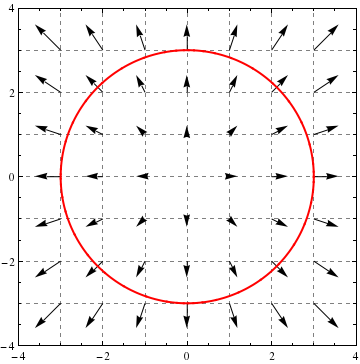
\includegraphics{circPosDivVecField.png}
  \end{image}
  Do you expect $\oint_C\vec{F} \dotp \d\vec{n}$ to be positive, zero,
  or negative?
  \begin{prompt}
    \begin{multipleChoice}
      \choice[correct]{positive}
      \choice{zero}
      \choice{negative}
    \end{multipleChoice}
  \end{prompt}
  \begin{question}
  Consider the following vector field $\vec{F}$ and curve $C$
  parameterized by $\vec{p}(t)$:
  \begin{image}
    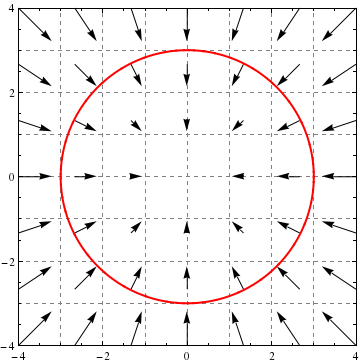
\includegraphics{circNegDivVecField.png}
  \end{image}
  Do you expect $\oint_C\vec{F} \dotp \d\vec{n}$ to be positive, zero,
  or negative?
  \begin{prompt}
    \begin{multipleChoice}
      \choice{positive}
      \choice{zero}
      \choice[correct]{negative}
    \end{multipleChoice}
  \end{prompt}  \begin{question}
  Consider the following vector field $\vec{F}$ and curve $C$
  parameterized by $\vec{p}(t)$:
  \begin{image}
    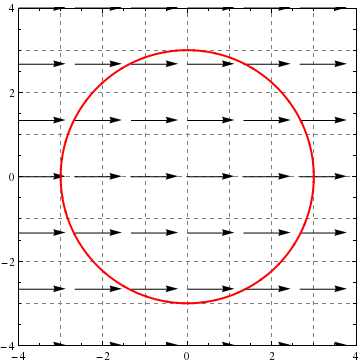
\includegraphics{circZeroDivVecField.png}
  \end{image}
  Do you expect $\oint_C\vec{F} \dotp \d\vec{n}$ to be positive, zero,
  or negative?
  \begin{prompt}
    \begin{multipleChoice}
      \choice{positive}
      \choice[correct]{zero}
      \choice{negative}
    \end{multipleChoice}
  \end{prompt}
  \end{question}
\end{question}
\end{question}

With our next example, we'll get our hands dirty.

\begin{example}
  Below we see a closed curve $C$ along with some representative field
  vectors of a vector field $\vec{F}$:
  \begin{image}
    \begin{tikzpicture}
      \begin{axis}%
        [
	  ymin=-.5,ymax=4.5,
	  xmin=-5.5,xmax=3.5,
          axis lines =middle, xlabel=$x$, ylabel=$y$,
          every axis y label/.style={at=(current axis.above origin),anchor=south},
          every axis x label/.style={at=(current axis.right of origin),anchor=west},
          grid=both,
          grid style={dashed, gridColor},
          xtick={-6,...,4},
          ytick={-1,...,5},
	]
      
        \addplot[penColor,thick,->] coordinates{
          (1,1.5) (2,2.5) 
        };
        \addplot[penColor,thick,->] coordinates{
          (0,2) (1,3) 
        };
        \addplot[penColor,thick,->] coordinates{
          (-1,2.5) (0,3.5) 
        };
        \addplot[penColor,thick,->] coordinates{
          (-2,3) (-1,4) 
        };

        
        \addplot[penColor,thick,->] coordinates{
          (-2.5,2.5) (-3.5,2.5) 
        };
        \addplot[penColor,thick,->] coordinates{
          (-3,2) (-4,2) 
        };
        \addplot[penColor,thick,->] coordinates{
          (-3.5,1.5) (-4.5,1.5) 
        };
        \addplot[penColor,thick,->] coordinates{
          (-4,1) (-5,1) 
        };

        
        \addplot[penColor,thick,->] coordinates{
          (-3,1) (-2,0) 
        };
        \addplot[penColor,thick,->] coordinates{
          (-2,1) (-1,0) 
        };
        \addplot[penColor,thick,->] coordinates{
          (-1,1) (0,0) 
        };
        \addplot[penColor,thick,->] coordinates{
          (0,1) (1,0) 
        };
        \addplot[penColor,thick,->] coordinates{
          (1,1) (2,0) 
        };
        \addplot[penColor,thick,->] coordinates{
          (2,1) (3,0) 
        };

        
        
        \addplot[penColor2,ultra thick] coordinates{
          (2,1) (-2,3) (-4,1) (2,1) (-2,3) 
        };
        \addplot[penColor2,ultra thick,->] coordinates{
          (2,1) (0,2) 
        };
        \addplot[penColor2,ultra thick,->] coordinates{
          (-2,3) (-3,2) 
        };
        \addplot[penColor2,ultra thick,->] coordinates{
          (-4,1) (-1,1) 
        };
        
      \end{axis}
    \end{tikzpicture}
  \end{image}
  Setting $\d x =1$ or $-1$ (depending on the direction of the curve),
  estimate:
  \[
  \oint_C \vec{F}\dotp\d\vec{n}
  \]
  \begin{explanation}
    If $\vec{F}(x,y)= \vector{M(x,y),N(x,y)}$, we have that:
    \[
    \oint_C \vec{F}\dotp\d\vec{n} = \oint_C -N(x,y)\d x + M(x,y)\d y
    \]
    We know that $|\d x|= \answer[given]{1}$, and $\d y = y'(x) \d x$. Now we'll compute
    \[
    \sum \left(-N(x,y) \d x + M(x,y) \d y\right)
    \]
    for each edge of the triangle above. For the bottom edge $\d x =
    \answer[given]{1}$ and $\d y = \answer[given]{0}$. So we have:
    \[
    \sum_{\mathrm{bottom}} \left(-N(x,y) \d x + M(x,y) \d y\right) = \answer[given]{6}
    \]
    Along the right edge, $\d x = \answer[given]{-1}$ and $\d y = \answer[given]{1/2}$. So
    \[
    \sum_{\mathrm{right}} \left(-N(x,y) \d x + M(x,y) \d y\right) = \answer[given]{6}
    \]
    Finally, along the left edge, $\d x = \answer[given]{-1}$ and $\d
    y = \answer[given]{-1}$. So
    \[
    \sum_{\mathrm{left}} \left(-N(x,y) \d x + M(x,y) \d y\right) = \answer[given]{4}.
    \]
    Hence we estimate
    \[
    \oint_C \vec{F}\dotp\d\vec{n} \approx\answer[given]{16}.
    \]
  \end{explanation}
\end{example}

\begin{example}
  Let $\vec{F}(x,y) = \vector{x,y}$ and let $C$ be the unit circle
  centered at the origin. Compute
  \[
  \oint_C \vec{F}\dotp \d\vec{n}
  \]
  \begin{explanation}
    The path $C$ can be parameterized by
    \begin{align*}
      x(\theta) &= \cos(\theta)\\
      y(\theta) &= \sin(\theta)
    \end{align*}
    with $0\le \theta\le 2\pi$. To compute the integral, write with me
    \begin{align*}
      \oint_C \vec{F}\dotp\d\vec{n} &= \int_0^{2\pi} F(x(\theta),y(\theta))\dotp \vector{y'(\theta),-x'(\theta)}\d \theta\\
      &= \int_0^{2\pi} \vector{\answer[given]{\cos(\theta)},\answer[given]{\sin(\theta)}}\dotp \vector{\answer[given]{\cos(\theta)},\answer[given]{\sin(\theta)}}\d \theta\\
      &= \int_0^{2\pi}\left(\cos^2(\theta)+\sin^2(\theta)\right)\d \theta\\
      &= \int_0^{2\pi} 1\d \theta\\
      &=\answer[given]{2\pi}.
    \end{align*}
  \end{explanation}
\end{example}


\section{Connections to Green's Theorem}

Finally, note that if $\vec{F}=\vector{M,N}$, then:
\begin{align*}
  \divergence \vec{F} &=\pp[M]{x} + \pp[N]{y}\\
  &=\curl\vector{-N,M}
\end{align*}
We also see that 
\begin{align*}
  \int_C \vector{-N,M} \d\vec{p} &= \int_C -N\d x+ M \d y\\
  &=\int_C \vec{F}\dotp\d\vec{n}
\end{align*}
this leads us to the \dfn{flux form of Green's Theorem}:

\begin{theorem}[Green's Theorem]\index{Green's Theorem}
  If the components of $\vec{F}:\R^2\to\R^2$ have continuous partial
  derivatives and $C$ is a boundary of a closed region $R$ and
  $\vec{p}(t) = \vector{x(t),y(t)}$ parameterizes $C$ in a
  counterclockwise direction with the interior on the left, and
  $\vec{n}(t) = \vector{y(t),-x(t)}$, then
  \[
  \iint_R \divergence\vec{F}\d A = \oint_C \vec{F}\dotp\d\vec{n} 
  \]
\end{theorem}

\begin{question}
  Let $\vec{F}$ be a vector field with $\divergence\vec{F} = 0$. Compute:
  \[
  \oint_C \vec{F}\dotp\d\vec{n}
  \begin{prompt}
    =\answer{0}
  \end{prompt}
  \]
\end{question}


\begin{question}
  Suppose that the curl of a vector field $\vec{F}:\R^2\to\R^2$ is
  constant, $\divergence\vec{F} = -4$.
  \begin{image}
    \begin{tikzpicture}
      \begin{axis}%
        [
	  ymin=-3,ymax=5,
	  xmin=-8,xmax=4,
          axis lines =middle, xlabel=$x$, ylabel=$y$,
          every axis y label/.style={at=(current axis.above origin),anchor=south},
          every axis x label/.style={at=(current axis.right of origin),anchor=west},
          grid=both,
          grid style={dashed, gridColor},
          xtick={-10,...,4},
          ytick={-6,...,6},
	]
        \addplot[penColor2,ultra thick,smooth] coordinates{
          (-6,3) (-1,3) (-1,1) (2,1) (2,-1)
        };

        \addplot[penColor4,ultra thick,smooth] coordinates{
          (2,-1) (-4,-1) (-4,1) (-6,1) (-6,3)
        };

        \addplot[penColor2,ultra thick,->] coordinates{
          (-1.05,1.5) (-1,1.7) 
        };

        \addplot[penColor4,ultra thick,->] coordinates{
          (-4,.6) (-4.1,.4) 
        };

        \fill[black,draw=black] (axis cs:-6,3) circle (2.5pt);

        \fill[black,draw=black] (axis cs:2,-1) circle (2.5pt);
        \node[above,penColor2] at (axis cs:-3,3) {$C_1$};
        \node[below,penColor4] at (axis cs:-2,-1.05) {$C_2$};
        
      \end{axis}
    \end{tikzpicture}
  \end{image}
  If
  \[
  \int_{C_1} \vec{F} \dotp\d \vec{n} = 20
  \]
  estimate
  \[
  \int_{C_2} \vec{F}\dotp\d\vec{n}
  \begin{prompt}
    = \answer{-108}
  \end{prompt}
  \]
  \begin{hint}
    Use Green's Theorem.
  \end{hint}
\end{question}



\end{document}
